\section{From Biophysics to Evolutionary Genetics: Statistical aspects of gene
regulation}

In this section we will be exploring with all the glorious details all the
derivations done by Michael Lassig in his beautiful review paper for BMC
Bioinformatics 2007.

\subsection{Biophysics of transcriptional regulation}
As an area of expertise in the lab, we are very familiar with the statistical
mechanics of gene regulation. The model we will use for this section has a list
of important assumptions that we will explicitly state:

(A) Given a transcription factor binding site of length $l$ with sequence
$\mathbf{a} = (a_1, a_2, \ldots, a_l)$, the binding energy can be assumed to be
a linear contribution of each base-pair, i.e.
\begin{equation}
  E(\mathbf{a}) = \sum_{i=1}^l \varepsilon_i (a_i),
\end{equation}
where $a_i \in \{A, G, C, T \}$.

(B) At each position there is a preferred base-pair $a_i^*$ such that
\begin{equation}
  \varepsilon_i (a_i^*) = \min_a \varepsilon_i(a).
\end{equation}
Therefore it is assumed that there is a unique {\it ground state} $\mathbf{a}^*
\equiv (a_1^*, a_2^*, \ldots, a_l^*)$ with minimum binding energy $E^* \equiv
E(\mathbf{a}^*)$.

(C) Mismatches cost energy differences of order $\varepsilon_i (a) -
\varepsilon_i (a_i^*) \sim 1-3 \; k_BT$.

We can make an order of magnitude estimate assuming a two-state system in which
a position has either the optimal base-pair $a_i^*$ or not, i.e.
\begin{equation}
\varepsilon_i (a) - \varepsilon_i (a_i^*) =
\begin{cases}
  \varepsilon & \text{if } a \neq a_i^*\\
  0 & \text{otherwise},
\end{cases}
\end{equation}
with $\varepsilon \sim 1 \; k_BT$. This approximation allows us to define the
binding energy of a sequence a s a function of the Hamming distance
$d(\mathbf{a}, \mathbf{a^*})$, i.e. the number of base-pair mismatches between
sequences,
\begin{equation}
  E(\mathbf{a}) = E^* + \varepsilon \cdot d(\mathbf{a}, \mathbf{a^*}).
\end{equation}

\fref[fig_tf_binding_ecoli](a) shows the energy distribution for a proposition
weight matrix (PMW) of {\it CRP} along the genome. As we can note the energies
seem to be randomly distributed. We can bin the energy as shown in
\fref[fig_tf_binding_ecoli](b). In the limit of large number of positions by the
law of large numbers we expect the distribution of the energies to be Gaussian.
We can compute the mean and variance of this expected Gaussian distribution by
scrambling the genome and computing the resulting binding energies.
\fref[fig_tf_binding_ecoli](b) shows this prediction align the actual genomic
data. It can be seen that for the most part the genome is indeed randomly
distributed. But, \manuelComment{as done by Lassig in a very confusing way}, we
can zoom into the low energy tail to find that there are several low energy
sequences that are overrepresented in the genome that might be there not by
chance.

\begin{figure}[h!]
	\centering 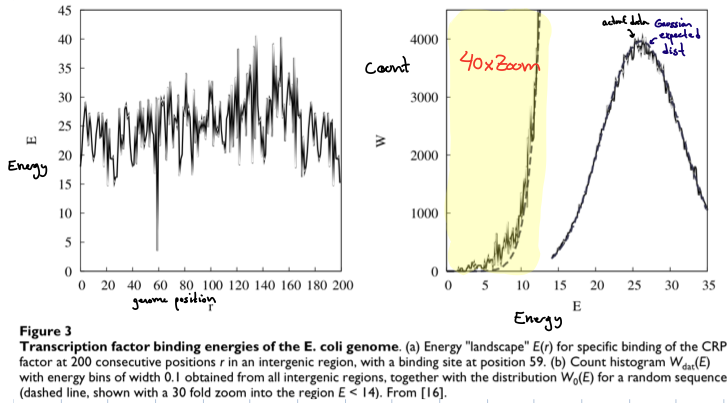
\includegraphics[scale=0.5]{../fig/lassig_2007/fig3.png}
	\caption{fig3}
  \label{fig_tf_binding_ecoli}
\end{figure}

\subsection{Thermodynamics of transcription factor binding}
\manuelComment{This section I don't feel is necessary in this document since
we are extremely familiar with that theory and my work is plagued with repeated
instances of this theory.}

\subsection{Sensitivity and genomic design of regulation}
Lassig goes into a very interesting and clever series of back-of-the-envelope
calculations about the design of regulatory binding sites given the physics of
transcription factor binding. The beautiful thing about these calculations is
that the numbers that come out are in perfect agreement with the inferred
binding energies for the {\it lac} repressor that we have always used. Let's go
through each of these calculations:

a) In a genome of length $\Nns \sim 5\times 10^6$ there must be at least one
{\it minimum energy} binding sites. If the genome was completely random
otherwise that would imply that the probability of finding the site would be
given by
\begin{equation}
  P(\mathbf{a}^*) = \prod_{i=1}^l P(a_i^*) = \left( {1 \over 4} \right)^l.
\end{equation}

The expected number of binding sites would then be constrained by
\begin{equation}
  \left\langle \text{\# binding sites} \right\rangle = \Nns P(\mathbf{a}^*)
   = \Nns \left( {1 \over 4} \right)^l \leq 1.
\end{equation}

Solving for the length of the binding site $l$ we find
\begin{align}
  \Nns &\leq 4^l\\
  \log \Nns &\leq l \log 4,
\end{align}
therefore
\begin{equation}
  l \geq {\log \Nns \over \log 4} \sim 10.
\end{equation}

b) If for a binding site of length $l$ there are $l$ possible sub-optimal
binding sites with Hamming distance 1, these sites should \textbf{not} suppress
binding to the optimal binding site. What this means is that it should hold
true that
\begin{equation}
  e^{-\beta E^*} \geq l e^{-\beta (E^* + \varepsilon)}.
\end{equation}
Solving for the energy difference $\varepsilon$ we find
\begin{align}
  -\beta E^* \leq \ln (l) - \beta (E^* + \varepsilon)\\
  \ln (l) \leq \beta \varepsilon \sim 2-3.
\end{align}
This implies that each base-pair should contribute with $\sim 2-3 \; k_BT$.

c) Finally the entirety of the {\it background genome} should not suppress
binding to the optimal binding site. Since we defined $E^*$ with respect to the
binding to the non-specific background it must hold true that
\begin{equation}
  e^{-\beta E^*} \geq \Nns e^{-\beta E_{NS}} = \Nns,
\end{equation}
since $E_{NS} = 0$ by definition.
This means that
\begin{equation}
  -\beta E^* \geq \log \Nns \sim 15.
\end{equation}
So the binding energy should be of order $-15 \; k_BT$ which is in perfect
agreement with the {\it lac} repressor.

\subsubsection{Programmability and evolvability of regulatory networks.}
In this section Lassig discusses very interesting points about the competition
between strong binding and evolvability.

If the cell wants to have a very specific binding of a transcription factor to
its corresponding functional binding site, the concept of {\it differential
programmability} would favor complicated molecular structures with long binding
sites to achieve large binding energies. However this competes with the {\it
evolvability} of the system via stochastic mutations.

Given the order-of-magnitude calculations in the previous section it seems that
indeed for the prokaryote case the gene regulatory machinery has almost single-
molecule sensitivity. This may result from a compromise between programmability
and evolvability, i.e. "binding sites are complicated enough to work."

\subsection{Bioinformatics of regulatory DNA.}
Lassig has come with a couple of methods to infer functional regulatory DNA that
takes into account the evolutionary history of the sequence. In this section we
will go through the logic of how to make these inferences.

\subsubsection{Markov model for background sequence}

Assuming that the genome is a Markov sequence with uniform probability for each
of the four nucleotides $P_o(a) = 1/4$, $a \in \{A, G, C, T \}$, we have that a
sequence $\mathbf{a}$ of length $k$ has a probability of occurring of the form
\begin{equation}
  P_o(\mathbf{a}) \prod_{i=1}^k P_o(a_i).
\end{equation}

Under the assumption that each base-pair contributes linearly to the total
binding site energy we can project the probability of sequences to the
\begin{equation}
  P_o(E) = \sum_{\mathbf{a}} P_o(\mathbf{a}) \delta(E - E(\mathbf{a})),
\end{equation}
where $\delta(x)$ is the delta function. What this equation syas is that the
probability of finding a sequence with binding energy $E$ is given by the sum
over all possible sequences, where the delta function guarantees that only the
sequences that happen to have the desired binding energy will contribute to the
sum. For example if only one sequence happened to have that specific energy, we
would sum over all possible sequences, but they would all be zero except for the
single sequence that maps to the desired energy. \fref[fig_tf_binding_ecoli](B)
shows that this model is very good at describing the genome.

\subsubsection{Probabilistic model for funcitonal sites.}

We can assume that the sequences $\mathbf{a} = (a_1, \ldots, a_l)$ on a binding
site are drawn from a different distribution $Q(\mathbf{a})$. We can then write
this distribution in terms of the non-specific distribution $P_o(\mathbf{a})$ as
\begin{equation}
  Q(\mathbf{a}) = P_o(\mathbf{a}) e^{S(\mathbf{a})},
\end{equation}
where $S(\mathbf{a})$ is called the {\it relative log-likelihood score} of the
distributions $P_o(\mathbf{a})$ and $Q(\mathbf{a})$. This quantity will be shown
to have an ipmortant evolutionary meaning, but for now we can trivially see that
this should be of the form
\begin{equation}
  S(\mathbf{a}) = \log \left( {Q(\mathbf{a}) \over P_o(\mathbf{a})} \right).
\end{equation}

For a single base-pair within the binding site we have that the probability of
a particular base $q_i(a)$, $i \in \{1, 2, \ldots, l\}$, $a \in \{A, G, C, T \}$
can be obtained by marginalizing the distribution $Q(\mathbf{a})$ as
\begin{equation}
  q_i(a) = \sum_{a_1} \sum_{a_2} \cdots \sum_{a_{i-1}}\sum_{a_{i+1}}
  \cdots \sum_{a_l} Q(a_1, a_2, \ldots, a_{i-1}, a_{i}, a_{i+1}, \ldots, a_l),
\end{equation}
or written in a compact form
\begin{equation}
  q_i(a) = \sum_{a_j \neq a_i} Q(\mathbf{a}).
\end{equation}
It is the set of these marginal distributions $q_i(a)$ that form the so-called
position weight matrix. If the score function $S(\mathbf{a})$ is additive in the
base-pair positions, i.e. $S(\mathbf{a}) = \sum_{i=1}^l s_i(a)$, then the
distribution $Q(\mathbf{a})$ has a factorized form
\begin{equation}
  Q(\mathbf{a}) = \prod_{i=1}^l q_i(a),
\end{equation}
with
\begin{equation}
  q_i(a) = P_o(a)\exp\left[ s_i(a) \right]
\end{equation}

We can again map the distribution into energies as
\begin{equation}
  Q(E) = \sum_{\mathbf{a}} Q(\mathbf{a}) \delta (E - E(\mathbf{a})),
\end{equation}
as well as the score function
\begin{equation}
  S(E) = \sum_{\mathbf{a}} S(\mathbf{a}) \delta (E - E(\mathbf{a})).
\end{equation}
Hence we can write
\begin{equation}
  Q(E) = P_o(E)\exp\left[ S(E) \right]
\end{equation}

\subsubsection{Bayesian model for genomic loci.}

We can now assume that the functional binding sites are distributed along the
genome with a small probability of occurring, $\lambda$. This allows us to
combine both distributions $P_o(\mathbf{a})$ and $Q(\mathbf{a})$ into something
called a Hidden Markov Model for a genomic sequence as
\begin{equation}
  W(\mathbf{a}) = \lambda Q(\mathbf{a}) + (1 - \lambda) P_o(\mathbf{a}),
\end{equation}
where $\lambda$ is known as the hidden variable.

The output of this model consists of pairs $(m, \mathbf{a})$ where first a
sequence is assigned as non-functional $(m=0)$ with probability $(1 - \lambda)$
or functional $(m=1)$ with probability $\lambda$. Based on this result the
sequence $\mathbf{a}$ is drawn out of $P_o(\mathbf{a})$ or $Q(\mathbf{a})$.
However we only have access to sequences $\mathbf{a}$ as data. The hidden
variable $m$ can be inferred from data using Bayes theorem as
\begin{equation}
  P(m \mid \mathbf{a}) = {P(\mathbf{a} \mid m) P(m) \over P(\mathbf{a})}.
\end{equation}
This an be rewritten as
\begin{equation}
  P(m \mid \mathbf{a}) = {P(\mathbf{a} \mid m) P(m) \over
  \sum_{m=0}^1 P(\mathbf{a} \mid m) P(m)}.
\end{equation}

This means that the probability of a given sequence $\mathbf{a}$ being
functional $\rho_f(\mathbf{a}) \equiv P(m=1\mid \mathbf{a})$ is given by
\begin{equation}
  \rho_f(\mathbf{a}) = {P(\mathbf{a} \mid m=1) P(m=1) \over
  P(\mathbf{a} \mid m=1) P(m=1) + P(\mathbf{a} \mid m=0) P(m=0)}.
\end{equation}
Writing this in terms of our distributions for specific and non-specific sites
gives
\begin{equation}
  \rho_f(\mathbf{a}) = {Q(\mathbf{a}) \cdot \lambda \over
  Q(\mathbf{a}) \cdot \lambda + P_o(\mathbf{a}) \cdot (1 - \lambda)}
\end{equation}

Rearranging terms we have
\begin{equation}
  \rho_f(\mathbf{a}) = {1 \over 1 + {(1 - \lambda) \over \lambda}
  {P_o(\mathbf{a}) \over Q(\mathbf{a})}}.
\end{equation}
Using the score function $S(\mathbf{a})$ gives
\begin{align}
  \rho_f(\mathbf{a}) &= {1  \over 1 + {(1 - \lambda) \over \lambda}
  \exp\left[ - S(\mathbf{a}) \right]},\\
  &= {1  \over 1 + \exp\left[ - S(\mathbf{a}) + \ln {(1 - \lambda) \over
  \lambda} \right]}.
\end{align}
When written in this form the function takes the form of a Fermi function with
threshold value $S(\mathbf{a}) = \ln {(1 - \lambda) \over \lambda}$ separating
the sequences likely to be functional from the non-functional ones.

This Bayesian model can again be projected onto energies
\begin{equation}
  W(E) = \lambda Q(E) + (1 - \lambda) P_o(E).
\end{equation}

\fref[fig_bayesian_dna] shows the application of this model to {\it CRP} on the
{\it E. coli} genome. This model seems to account for the data displayed.

\begin{figure}[h!]
	\centering 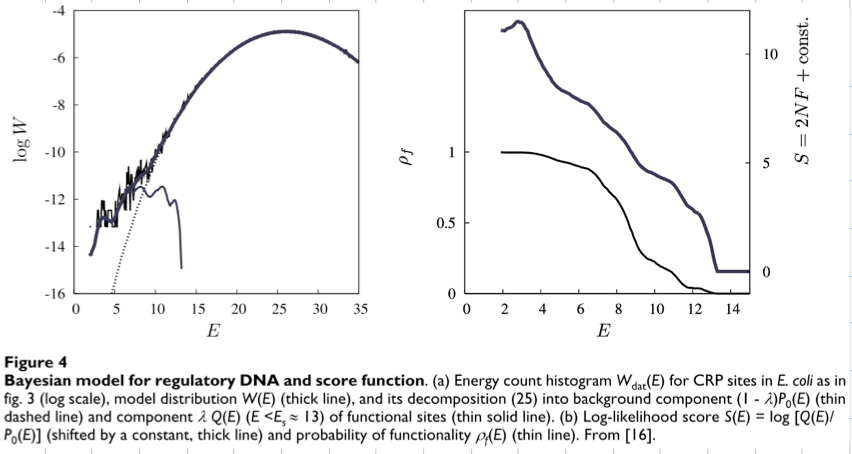
\includegraphics[scale=0.5]{../fig/lassig_2007/fig4.png}
	\caption{fig3}
  \label{fig_bayesian_dna}
\end{figure}
